\chapter{Interfacing a Pushbutton}
\thispagestyle{empty}
\label{pushbutton}

\newcommand{\LocPushfig}{\Origin/user-code/push/figures}
\newcommand{\LocPushscicode}{\Origin/user-code/push/scilab}
\newcommand{\LocPushscibrief}{Orign/user-code/push/scilab}
\newcommand{\LocPushardcode}{\Origin/user-code/push/arduino}
\newcommand{\LocPushardbrief}{Orign/user-code/push/arduino}

\newcommand{\LocPushbrief}{Orign/user-code/push/code}

In this experiment we will learn about digital input in arduino. We will read the status of pushbutton switch connected to Arduino using scilab-arduino toolbox. This status can be used  to perform different operations. Monitoring status using digital logic is very basic and important task in many applications. This experiment will enable you to do the same. 

\section{Preliminaries}
Pushbutton is a simple switch which is used to connect/disconnect circuit. When push-button interfaced with microcontroller circuit is pressed, it changes logic level of the micro-controller pin connected to its terminal. 

After pressing the button two terminals get electrically connected (short) and thus current flows through the pushbutton. As you might expect, there is limit to maximum current that could flow through pushbutton. This maximum current is also called as rated current and is provided by manufacturer in the datasheet.

\section{Reading a Pushbutton from the Arduino IDE}

\subsection{Reading values from Arduino through Scilab}
In this section we will see how arduino conveys digital value to the scilab software installed in the computer. This is done by Scilab-arduino toolbox we are using. But at root level, digital data transfer between Arduino and Scilab happens because of RS232 serial communication.  

\subsubsection{RS232 serial communication}
Serial communication is wired communication standard where 2 computing units talk with each other using two wires. RS232 is one of the widely used standard of  data transfer. In this, data transfer over each wire takes place sequentially with 1 bit at a time. Each unit has separate receive and transmit connection, thus it s full duplex mode of communication. All Arduino boards have special hardware called universal asynchronous receiver transmitter (UART) to enable fast RS232 serial communication. RS232 serial transmit (Tx) and serial receive (Rx) connections are provided at digital pin 1 and 0 respectively. With the serial-USB adapter, this serial port communicates with computer with scilab installed. Scilab-arduino toolbox uses this serial port in the backend. Some of the Arduino variants like arduino mega provide multiple inbuilt serial ports. 

To start a serial communication few configuration parameters need to be set. They must be same for both the units involved in communication. Parameters needed for serial communication are Baud rate, start bit, stop bit, parity type, etc.

\subsection{Connections}
Pushbutton is connected  to the digital pin 4 of arduino using shield given in kit. It has 2 pair of terminals. Each pair is electrically connected. When pushbutton is pressed all the terminals become short.  

\subsection{Block diagram}

\section{Experiment: Reading digital input}
In this experiment we will read the pushbutton status in scilab console. We have to write a cmd\_digital\_read function. The general form of this function is given as:
\begin{lstlisting}
ans=cmd_digital_in(1, pin)
\end{lstlisting}


\section{Reading a Pushbutton from the Arduino IDE}
\subsection{Scilab script}



\subsection{Xcos implementation}
The Xcos implementation for this experiment is shown in the \figref{pushbuttonstat}.

\begin{figure}
\centering
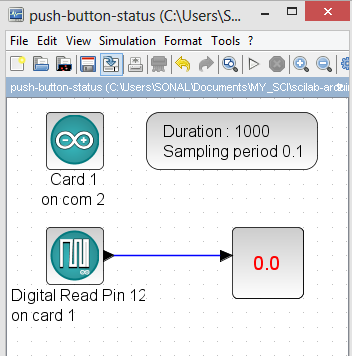
\includegraphics[width=\smfig]{\LocPushfig/push-button-status.png}
\caption{Xcos diagram}
\label{fig:pushbuttonstat}
\end{figure}

\subsubsection{Output}
Using serial connection between Arduino and scilab,  digital status of the pushbutton is observed on scilab console. In xcos, graphical plot of the same can be observed. When user presses the button, change in the logic value from low to high can be observed. 


\section{Experiment: Controlling LED using pushbutton}
In this experiment, we will learn to switch on/off LED using pushbutton. Here both the peripherals LED and button works with digital logic. Thus LED digital output is decided by the digital input received from pushbutton. Scilab code for direct implementation in scilab-arduino toolbox is mentioned below.

\subsection{Scilab script}



\subsection{Xcos implementation}
The Xcos implementation for this experiment is shown in the \figref{pushbuttonstat}.

\begin{figure}
\centering
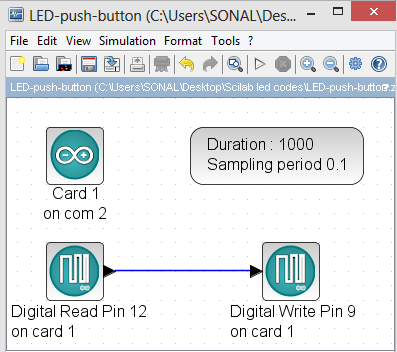
\includegraphics[width=\smfig]{\LocPushfig/led-push-button.png}
\caption{Xcos diagram}
\label{fig:ledpushbutton}
\end{figure}


\subsubsection{Output}
Each time user presses button, LED on the shield is switched on. When button is released LED is switched off again. Here we note that digital logic level of the Arduino pin connected to pushbutton changes only for the time button is being pressed. 


\subsubsection{Troubleshooting}
You can check whether pushbutton is working correctly or not by checking connections. If pushbutton is working correctly, all the 4 terminals show electrical short. You can check this with digital multimeter (DMM). When pushbutton is released 2 pair of terminals are not connected to the other 2 terminals on the other side. However, each pair is still shorted.


\subsection{Exercise}

\section{Arduino Code}
\lstset{style=mystyle}
\label{sec:push-arduino-code}
\addtocontents{cod}{\protect\addvspace{\codclr}}

\begin{ardcode}
\ccaption{Turning on the blue LED}{Turning on the blue LED.  Available
  at \LocPushardbrief/push-button-status/push-button-status.ino}
\label{ard:push-status}
\lstinputlisting{\LocPushardcode/push-button-status/push-button-status.ino}
\end{ardcode}

\begin{ardcode}
\ccaption{Turning on the blue LED}{Turning on the blue LED.  Available
  at \LocPushardbrief/led-push-button/led-push-button.ino}
\label{ard:led-blue}
\lstinputlisting{\LocPushardcode/led-push-button/led-push-button.ino}
\end{ardcode}



\section{Scilab Code}
\label{sec:push-scilab-code}
\addtocontents{cod}{\protect\addvspace{\codclr}}
\begin{scicode}
\ccaption{Interfacing a Pushbutton}
{Read and display the LDR values.  Available at
  \LocPushscibrief/push-button-status.sce.} 
\label{sci:push-100}
\lstinputlisting{\LocPushscicode/push-button-status.sce}
\end{scicode}

\begin{scicode}
\ccaption{Interfacing a Pushbutton}
{Change the LED state depending on the LDR values. Available at
  \LocPushscibrief/led-push-button.sce.} 
\label{sci:push-200}
\lstinputlisting{\LocPushscicode/led-push-button.sce}
\end{scicode}
